\documentclass[12pt,a4paper]{article}

% --- Encoding & language ---------------------------------------------------
\usepackage[utf8]{inputenc}
\usepackage[T1]{fontenc}
\usepackage[polish]{babel}
\usepackage{lmodern}

% --- Layout ----------------------------------------------------------------
\usepackage[a4paper,margin=2.5cm]{geometry}
\usepackage{setspace}
\setstretch{1.18}
\usepackage{microtype}
\usepackage{parskip}

% --- Math, tables, figures -------------------------------------------------
\usepackage{amsmath,amssymb}
\usepackage{graphicx}
\usepackage{booktabs}
\usepackage{array}
\usepackage{caption}
\captionsetup{font=small,labelfont=bf}
\usepackage{float}

% --- References & links ----------------------------------------------------
\usepackage[hidelinks]{hyperref}

\graphicspath{{figures/}}

% --- Generated macros (numbers produced by the experiment) -----------------
% If the pipeline has been run, load the real numbers; otherwise fall back to
% neutral placeholders so the document still compiles.
\IfFileExists{generated/macros.tex}{%
  \newcommand{\resDataSource}{cicids2018}
\newcommand{\resNTotal}{114\,621}
\newcommand{\resNTrain}{73\,356}
\newcommand{\resNVal}{18\,340}
\newcommand{\resNTest}{22\,925}
\newcommand{\resNFeatures}{68}
\newcommand{\resNClasses}{15}
\newcommand{\resBestFOneModel}{CNN 1D}
\newcommand{\resBestFOne}{0.913}
\newcommand{\resRFFOne}{0.912}
\newcommand{\resRFAUC}{0.968}
\newcommand{\resBestDeepModel}{CNN 1D}
\newcommand{\resBestDeepFOne}{0.913}
\newcommand{\resRFTrainTime}{4.16}
\newcommand{\resBestDeepTrainTime}{171.74}%
}{%
  \newcommand{\resDataSource}{synthetic}
  \newcommand{\resNTotal}{--}
  \newcommand{\resNTrain}{--}
  \newcommand{\resNVal}{--}
  \newcommand{\resNTest}{--}
  \newcommand{\resNFeatures}{--}
  \newcommand{\resNClasses}{--}
  \newcommand{\resBestFOneModel}{--}
  \newcommand{\resBestFOne}{--}
  \newcommand{\resRFFOne}{--}
  \newcommand{\resRFAUC}{--}
  \newcommand{\resBestDeepModel}{--}
  \newcommand{\resBestDeepFOne}{--}
  \newcommand{\resRFTrainTime}{--}
  \newcommand{\resBestDeepTrainTime}{--}
}

\begin{document}

\begin{titlepage}
\centering

\vspace*{1.5cm}
{\large Praca projektowa (inżynierska)\par}
\vspace{0.5cm}
{\large\itshape Uczenie maszynowe w cyberbezpieczeństwie chmury\par}

\vfill

{\Huge\bfseries Porównanie skuteczności metod uczenia głębokiego i lasów losowych w prognozowaniu naruszeń danych w chmurze\par}

\vspace{1.0cm}
{\large\itshape Comparison of deep learning methods and random forests in forecasting cloud data breaches\par}

\vfill

\begin{flushright}
\begin{tabular}{rl}
\textbf{Temat:} & Detekcja i prognozowanie naruszeń danych \\
\textbf{Metody:} & Lasy losowe vs. sieci głębokie (MLP, CNN, LSTM) \\
\textbf{Zbiór danych:} & CSE-CIC-IDS2018 / dane syntetyczne \\
\end{tabular}
\end{flushright}

\vfill

{\large \today\par}

\end{titlepage}


\newpage
\section*{Streszczenie}
\addcontentsline{toc}{section}{Streszczenie}

Coraz więcej danych trafia do chmury obliczeniowej, a wraz z nimi rośnie ryzyko
ich naruszenia. Celem tej pracy jest sprawdzenie, jak dobrze metody uczenia
maszynowego potrafią wykrywać ataki prowadzące do takich naruszeń, oraz
porównanie dwóch popularnych podejść: klasycznego \emph{lasu losowego} oraz
\emph{sieci głębokich} (MLP, CNN i LSTM). Zadanie sformułowano jako rozpoznawanie
złośliwych połączeń sieciowych --- model decyduje, czy dane połączenie to ruch
normalny, czy atak.

W ramach projektu zbudowano kompletny, samodzielnie uruchamialny program w
języku Python, który wczytuje dane, przygotowuje je, trenuje wszystkie modele i
porównuje ich wyniki. Eksperyment przeprowadzono na danych \texttt{\resDataSource},
opartych na zbiorze CSE-CIC-IDS2018 --- ruchu sieciowym zebranym na
infrastrukturze chmurowej. Modele oceniono zarówno pod kątem skuteczności
(m.in.\ wykrywalność ataków i liczba fałszywych alarmów), jak i kosztu (czas
uczenia oraz złożoność).

Wyniki pokazują, że najlepszy model głęboki (\resBestDeepModel,
F1\,=\,\resBestDeepFOne) osiąga nieco wyższą skuteczność niż las losowy
(F1\,=\,\resRFFOne), ale kosztem znacznie dłuższego uczenia. Las losowy okazuje
się najlepszym kompromisem między jakością a kosztem, a bardziej skomplikowane
sieci (CNN, LSTM) nie dają tutaj wyraźnej przewagi.

\medskip
\noindent\textbf{Słowa kluczowe:} bezpieczeństwo chmury, naruszenie danych,
wykrywanie ataków, uczenie maszynowe, las losowy, sieci głębokie,
CSE-CIC-IDS2018.


\newpage
\tableofcontents

\newpage
\section{Wstęp}
\label{sec:wstep}

\subsection{Wprowadzenie}

Trudno dziś wyobrazić sobie firmę, która nie korzysta z chmury obliczeniowej.
Poczta, dokumenty, bazy danych, całe aplikacje --- wszystko to coraz częściej
działa na serwerach wynajmowanych od dostawców takich jak Amazon, Microsoft czy
Google. Razem z usługami do chmury trafiają jednak dane, w tym te najbardziej
wrażliwe. To czyni chmurę łakomym kąskiem dla cyberprzestępców, a \emph{naruszenie
danych} --- czyli ich wyciek lub kradzież --- jednym z najbardziej kosztownych
incydentów, jakie mogą spotkać organizację.

Klasyczne zabezpieczenia, oparte na gotowych ,,sygnaturach'' znanych ataków,
coraz słabiej radzą sobie z nowymi zagrożeniami i z ogromną skalą ruchu w
chmurze. Dlatego dużą nadzieję pokłada się w \emph{uczeniu maszynowym} --- czyli
w modelach, które samodzielnie uczą się rozpoznawać złośliwą aktywność na
podstawie wcześniejszych przykładów. Wśród wielu dostępnych metod szczególnie
wyróżniają się dwie: \emph{lasy losowe} (sprawdzona, ,,klasyczna'' technika) oraz
\emph{uczenie głębokie} (nowsze, oparte na sieciach neuronowych). Obie potrafią
osiągać świetne wyniki, ale różnią się złożonością, kosztem i tym, jak łatwo
zrozumieć ich decyzje.

\subsection{Cel pracy}

Celem pracy jest \textbf{porównanie skuteczności metod uczenia głębokiego i
lasów losowych w wykrywaniu (prognozowaniu) naruszeń danych w chmurze}. Przez
,,prognozowanie naruszenia'' rozumiemy rozpoznawanie pojedynczych połączeń
sieciowych jako normalnych lub złośliwych --- wykrycie podejrzanego połączenia
jest bowiem wczesnym ostrzeżeniem przed pełnym wyciekiem danych.

Chcemy w szczególności odpowiedzieć na trzy pytania:
\begin{enumerate}
  \item Które podejście --- las losowy czy sieci głębokie --- skuteczniej
        wykrywa ataki?
  \item Ile kosztuje (pod względem czasu uczenia i działania) każde z nich i czy
        wyższa skuteczność jest warta tego kosztu?
  \item Czy bardziej rozbudowane sieci (CNN, LSTM) są lepsze od prostej sieci
        MLP na danych opisujących ruch sieciowy?
\end{enumerate}

\subsection{Zakres i sposób realizacji}

Projekt ma charakter zarówno teoretyczny, jak i praktyczny. Część praktyczna to
napisany od podstaw program w Pythonie, który realizuje cały eksperyment ---
od przygotowania danych, przez uczenie pięciu modeli, po obliczenie wyników i
wygenerowanie wykresów. Wszystkie liczby i rysunki w sprawozdaniu pochodzą
bezpośrednio z tego programu, dzięki czemu treść jest zgodna z faktycznymi
wynikami.

\subsection{Układ dokumentu}

Dalsza część pracy ma typowy układ: w rozdziale~\ref{sec:problem} przybliżamy
problem bezpieczeństwa danych w chmurze, w rozdziale~\ref{sec:podstawy}
opisujemy porównywane metody, rozdział~\ref{sec:metodyka} przedstawia sposób
przeprowadzenia eksperymentu, rozdział~\ref{sec:realizacja} prezentuje i omawia
wyniki, a rozdział~\ref{sec:wnioski} zawiera wnioski oraz pomysły na dalsze
prace.

\section{Bezpieczeństwo danych w chmurze obliczeniowej i sformułowanie problemu}
\label{sec:problem}

\subsection{Specyfika zagrożeń w środowisku chmurowym}

Chmura obliczeniowa zmieniła sposób, w jaki firmy przechowują i przetwarzają
dane. Zamiast utrzymywać własne serwerownie, organizacje wynajmują zasoby od
dostawców takich jak Amazon Web Services, Microsoft Azure czy Google Cloud.
Wygoda i oszczędność mają jednak swoją cenę --- dane wielu klientów żyją na tej
samej, współdzielonej infrastrukturze, dostępnej przez sieć z dowolnego miejsca
na świecie. To sprawia, że chmura jest atrakcyjnym celem dla atakujących.

Warto pamiętać o tzw.\ \textbf{modelu współdzielonej odpowiedzialności}: dostawca
chmury dba o bezpieczeństwo samej infrastruktury, ale za poprawną konfigurację,
kontrolę dostępu i ochronę własnych danych odpowiada już klient. W praktyce
ogromna część głośnych wycieków danych z chmury wynikała nie z włamania do
serwerów dostawcy, lecz z błędów po stronie użytkownika --- źle ustawionych
uprawnień, otwartych ,,kubełków'' z danymi czy przejętych kont. Dodatkowo skala
i zmienność ruchu w chmurze są tak duże, że ręczne pilnowanie bezpieczeństwa
przestaje być możliwe.

\subsection{Pojęcie naruszenia danych}

\textbf{Naruszenie danych} (ang.\ \emph{data breach}) to sytuacja, w której
dane trafiają w niepowołane ręce --- zostają wykradzione, ujawnione lub zmienione
bez uprawnienia. Konsekwencje bywają dotkliwe: kary finansowe (np.\ na gruncie
RODO), utrata zaufania klientów i realne straty. Co gorsza, naruszenia często
pozostają niewykryte przez wiele tygodni, co daje atakującym czas na wyrządzenie
dużych szkód.

W środowisku chmurowym najczęstsze drogi prowadzące do naruszenia to m.in.:
\begin{itemize}
  \item \textbf{przejęcie kont} --- np.\ zgadywanie haseł metodą brute force do
        usług logowania;
  \item \textbf{eksfiltracja danych} --- niepostrzeżone wyprowadzanie danych na
        zewnątrz, często ukryte w pozornie zwykłym ruchu;
  \item \textbf{ataki DoS/DDoS} --- zalewanie usług ruchem, czasem jako zasłona
        dymna dla innych działań;
  \item \textbf{infiltracja i ruch boczny} --- po zdobyciu przyczółka atakujący
        przemieszcza się w infrastrukturze ofiary;
  \item \textbf{botnety} oraz \textbf{ataki na aplikacje webowe} (np.\ SQL
        injection), które również prowadzą do wycieku danych.
\end{itemize}

Wszystkie te działania mają jedną wspólną cechę: zostawiają ślad w \emph{ruchu
sieciowym}. Analizując ten ruch, można wychwycić podejrzaną aktywność, zanim
przerodzi się ona w pełne naruszenie.

\subsection{Od wykrywania ataków do prognozowania naruszeń}

Naruszenie danych rzadko jest pojedynczym zdarzeniem --- to zwykle finał całego
łańcucha działań: rozpoznanie, włamanie, eskalacja uprawnień, wreszcie kradzież
danych. Jeśli uda się wykryć wczesne ogniwa tego łańcucha (np.\ nietypowe
połączenie świadczące o skanowaniu lub łamaniu haseł), można zareagować, \emph{zanim}
dojdzie do wycieku. W tym sensie wykrycie ataku pełni rolę \emph{prognostyczną}
--- jest wczesnym sygnałem ostrzegawczym. Dlatego w tej pracy ,,prognozowanie
naruszenia'' utożsamiamy z rozpoznawaniem złośliwych połączeń sieciowych.

\subsection{Sformułowanie zadania klasyfikacji}

Zadanie sprowadza się do prostego pytania zadawanego dla każdego połączenia
sieciowego: \emph{czy to zwykły, normalny ruch, czy raczej atak?} Każde
połączenie opisujemy zestawem liczb --- na przykład jak długo trwało, ile
pakietów i bajtów przesłano, jak często, jakie flagi sieciowe się pojawiły.
Na podstawie tych cech model ma przykleić jedną z dwóch etykiet: \emph{ruch
normalny} albo \emph{atak}. Model uczy się tej umiejętności na historycznych
przykładach, dla których wiadomo, co było czym. Jest to więc klasyczne zadanie
\textbf{klasyfikacji} --- a ponieważ dane zawierają też informację o rodzaju
ataku, możliwa jest dodatkowo analiza poszczególnych typów zagrożeń.

\subsection{Wyzwania badawcze}

Wykrywanie naruszeń nie jest proste z kilku praktycznych powodów:
\begin{itemize}
  \item \textbf{Ataki są rzadkie.} W normalnym ruchu tonie garstka złośliwych
        połączeń. Model łatwo wpada w pułapkę uznawania ,,wszystkiego za
        normalne'' i przeocza zagrożenia.
  \item \textbf{Nie każdy błąd kosztuje tyle samo.} Przeoczenie ataku jest
        zwykle znacznie groźniejsze niż fałszywy alarm --- dlatego zależy nam
        przede wszystkim na wykrywalności (czułości).
  \item \textbf{Złośliwość kryje się w kombinacjach.} Pojedyncza cecha rzadko
        zdradza atak; dopiero ich zestawienie tworzy podejrzany obraz, co
        wyklucza najprostsze, ,,liniowe'' metody.
  \item \textbf{Liczy się szybkość i koszt.} W chmurze model trzeba często
        dotrenowywać i stosować na bieżąco do ogromnych ilości ruchu, więc nie
        może być zbyt kosztowny obliczeniowo.
\end{itemize}

Te właśnie wyzwania kształtują dobór metod i sposób ich oceny, co opisujemy w
kolejnych rozdziałach.

\section{Podstawy teoretyczne zastosowanych metod}
\label{sec:podstawy}

W tym rozdziale opisano --- w sposób możliwie przystępny, bez zagłębiania się w
formalizm matematyczny --- dwie rodziny metod, które porównujemy: las losowy
oraz sieci głębokie. Celem jest zrozumienie, \emph{jak} działają i \emph{czym}
się różnią, bo to te różnice decydują o ich przydatności w ochronie danych w
chmurze.

\subsection{Las losowy}

Punktem wyjścia jest \emph{drzewo decyzyjne}. Można je sobie wyobrazić jako
listę pytań typu ,,czy liczba pakietów w połączeniu przekracza pewien próg?''.
Odpowiadając na kolejne pytania, schodzimy w dół drzewa aż do liścia, który
mówi: ,,to ruch normalny'' albo ,,to atak''. Pojedyncze drzewo jest jednak
kapryśne --- drobna zmiana danych potrafi je całkowicie przebudować, przez co
łatwo się ,,przeucza'' i słabo radzi sobie z nowymi przypadkami.

\emph{Las losowy}~\cite{breiman2001random} rozwiązuje ten problem prostą, ale
skuteczną sztuczką: zamiast jednego drzewa buduje ich setki, a każde uczy na
nieco innym, losowym wycinku danych i cech. Decyzja końcowa zapada przez
\emph{głosowanie} --- jeśli większość drzew uznaje połączenie za atak, takim
jest klasyfikowane. Dzięki temu, że drzewa popełniają różne błędy, ich
uśrednienie daje wynik znacznie stabilniejszy niż każde drzewo z osobna.

Las losowy ma kilka cech, które czynią go popularnym w cyberbezpieczeństwie:
nie wymaga skalowania danych, dobrze radzi sobie ze złożonymi zależnościami
między cechami, szybko się uczy i --- co istotne dla analityka --- potrafi
wskazać, \textbf{które cechy} były najważniejsze przy podejmowaniu decyzji.

\subsection{Sieci głębokie}

\emph{Sieć neuronowa} to model luźno inspirowany działaniem mózgu. Składa się z
warstw ,,neuronów'', z których każdy łączy informacje z poprzedniej warstwy i
przekazuje wynik dalej. Określenie \emph{głęboka} oznacza po prostu, że warstw
jest wiele --- dzięki temu sieć stopniowo buduje coraz bardziej złożone wzorce:
od prostych zależności po abstrakcyjne ,,sygnatury'' złośliwej aktywności.
Sieć uczy się, wielokrotnie oglądając przykłady i samodzielnie korygując swoje
,,wewnętrzne pokrętła'' tak, aby coraz rzadziej się mylić.

W pracy porównujemy trzy architektury sieci:

\paragraph{MLP (perceptron wielowarstwowy).} Najprostsza i najbardziej klasyczna
sieć w pełni połączona. Traktuje dane jak zwykłą tabelę liczb i jest naturalnym
wyborem dla danych opisujących połączenia sieciowe.

\paragraph{CNN 1D (sieć konwolucyjna).} Sieć, która ,,przesuwa okienko'' po
danych i wyszukuje powtarzające się, lokalne wzorce~\cite{lecun1998gradient}.
Sprawdza się świetnie w analizie obrazów czy sygnałów; tutaj sprawdzamy, czy
podobne podejście pomaga w danych o ruchu sieciowym.

\paragraph{LSTM (sieć rekurencyjna).} Sieć z ,,pamięcią'', zaprojektowana do
danych o charakterze sekwencji~\cite{hochreiter1997long}. Potrafi uwzględniać
kolejność i zależności między kolejnymi elementami, dlatego włączamy ją do
porównania, by sprawdzić, czy modelowanie ,,sekwencyjności'' cech przynosi
jakąkolwiek korzyść.

\subsection{Miary oceny skuteczności}

Sama ,,dokładność'' (odsetek poprawnych decyzji) bywa myląca, gdy ataki są
rzadkie --- model, który wszystko uzna za ruch normalny, może mieć wysoką
dokładność, a jednocześnie nie wykryć żadnego włamania. Dlatego patrzymy na
kilka uzupełniających się miar, opisanych tu zwykłym językiem:

\begin{itemize}
  \item \textbf{Precyzja} --- spośród połączeń oznaczonych jako atak, jaki
        odsetek faktycznie był atakiem. Niska precyzja oznacza wiele
        \emph{fałszywych alarmów}, które męczą zespół bezpieczeństwa.
  \item \textbf{Czułość} (ang.\ \emph{recall}) --- spośród wszystkich
        prawdziwych ataków, ile udało się wykryć. Niska czułość oznacza
        \emph{przeoczone włamania} --- najgroźniejszy rodzaj błędu.
  \item \textbf{F1} --- jedna liczba godząca precyzję i czułość; wygodna do
        porównań.
  \item \textbf{ROC-AUC} i \textbf{PR-AUC} --- miary opisujące jakość modelu
        niezależnie od ustawionego ,,progu czułości''; im bliżej $1{,}0$, tym
        lepiej.
\end{itemize}

W kontekście ochrony danych w chmurze szczególnie zależy nam na \emph{wysokiej
czułości} (żeby nie przeoczyć naruszenia) przy rozsądnej precyzji (żeby nie
zasypać analityków fałszywymi alarmami).

\subsection{Przegląd literatury}

Wykrywanie włamań metodami uczenia maszynowego to dobrze zbadany temat.
Najczęściej wykorzystuje się publiczne zbiory danych, takie jak
NSL-KDD~\cite{tavallaee2009detailed}, UNSW-NB15~\cite{moustafa2015unsw} czy
CIC-IDS2017/CSE-CIC-IDS2018 przygotowane przez Canadian Institute for
Cybersecurity~\cite{sharafaldin2018toward}. Co ciekawe, w wielu badaniach metody
oparte na drzewach (jak las losowy) okazują się równie dobre lub lepsze od sieci
głębokich, gdy dane mają postać \emph{tabeli} --- a tak właśnie wyglądają cechy
połączeń sieciowych~\cite{grinsztajn2022why}. Sieci głębokie błyszczą przede
wszystkim tam, gdzie dane są surowe i mają wyraźną strukturę (obrazy, dźwięk,
tekst). Niniejsza praca sprawdza, czy ta obserwacja potwierdza się również w
naszym, ,,chmurowym'' zadaniu.

\section{Metodyka badawcza}
\label{sec:metodyka}

\subsection{Ogólny schemat eksperymentu}

Aby porównanie było uczciwe, wszystkie modele uczono i testowano \emph{na tych
samych danych} i oceniano \emph{tymi samymi miarami}. Cały eksperyment przebiega
według prostego scenariusza:

\begin{enumerate}
  \item wczytanie danych (rzeczywisty zbiór CSE-CIC-IDS2018 lub --- gdy nie jest
        dostępny --- dane syntetyczne),
  \item przygotowanie danych (oczyszczenie, ujednolicenie, podział na zbiory),
  \item wytrenowanie pięciu modeli: regresji logistycznej, lasu losowego oraz
        sieci MLP, CNN i LSTM,
  \item ocena każdego modelu (skuteczność oraz czas uczenia i działania),
  \item zebranie wyników w postaci tabel i wykresów.
\end{enumerate}

\subsection{Zbiór danych}

Głównym zbiorem danych jest \textbf{CSE-CIC-IDS2018} --- duży, publicznie
dostępny zbiór ruchu sieciowego zebranego na chmurowej infrastrukturze AWS przez
Canadian Institute for Cybersecurity~\cite{sharafaldin2018toward}. Zawiera on
zarówno ruch normalny, jak i różne typy ataków (m.in.\ łamanie haseł, DoS/DDoS,
ataki na aplikacje webowe, infiltrację oraz botnety). Każde połączenie opisane
jest kilkudziesięcioma cechami liczbowymi --- na przykład czasem trwania, liczbą
i rozmiarem przesłanych pakietów, tempem transmisji czy licznikami flag
sieciowych.

Pełny zbiór waży kilka gigabajtów, dlatego program wczytuje go w częściach i
losowo próbkuje, biorąc porcję danych z każdego dnia (każdy dzień zawiera inne
typy ataków). Dla zachowania pełnej powtarzalności --- gdyby ktoś chciał
uruchomić projekt bez pobierania wielkich plików --- przygotowano też
\emph{generator danych syntetycznych} o zbliżonej charakterystyce. Program
automatycznie korzysta z danych rzeczywistych, jeśli są dostępne, a w przeciwnym
razie z danych syntetycznych.

W opisywanym eksperymencie wykorzystano dane \texttt{\resDataSource}: łącznie
\resNTotal{} połączeń opisanych \resNFeatures{} cechami. Rozkład klas (widoczna
przewaga ruchu normalnego, typowa dla takich zadań) przedstawia
rys.~\ref{fig:class-dist}.

\begin{figure}[H]
\centering
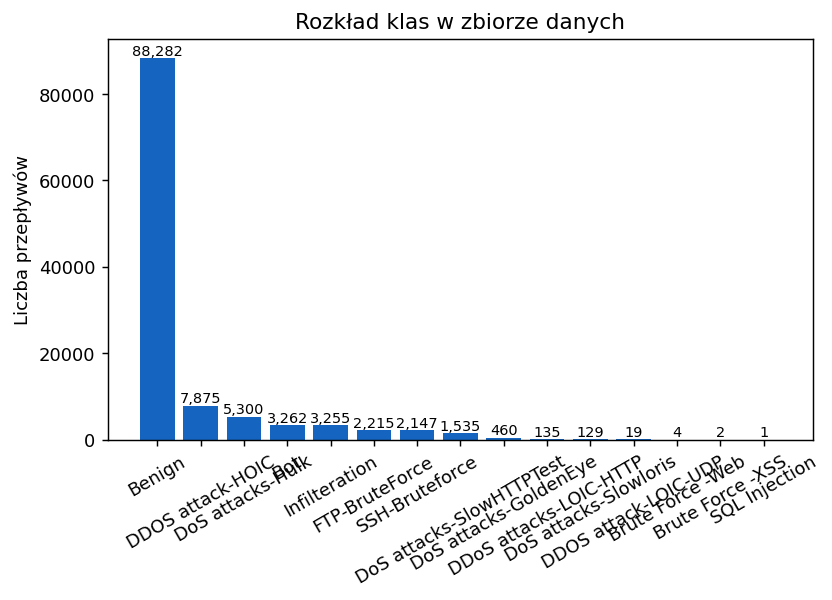
\includegraphics[width=0.8\textwidth]{class_distribution.png}
\caption{Rozkład klas w danych. Ruch normalny wyraźnie dominuje nad atakami ---
to częste wyzwanie w wykrywaniu zagrożeń.}
\label{fig:class-dist}
\end{figure}

\subsection{Przetwarzanie wstępne danych}

Surowe dane wymagają porządków. Etap przygotowania obejmuje:
\begin{itemize}
  \item usunięcie kolumn nieprzydatnych do klasyfikacji (adresy IP, porty,
        znaczniki czasu) oraz kolumn o stałej wartości;
  \item poprawienie brakujących i błędnych wartości (np.\ wartości
        nieskończonych powstających przy dzieleniu);
  \item zamianę etykiet na prostą postać: ruch normalny lub atak (zachowano
        też informację o konkretnym typie ataku do celów poglądowych);
  \item ujednolicenie skali cech, tak aby duże liczby nie ,,zagłuszały''
        mniejszych --- co jest ważne zwłaszcza dla sieci neuronowych;
  \item podział danych na trzy części: uczącą, walidacyjną (do strojenia) i
        testową (do końcowej, uczciwej oceny).
\end{itemize}
Podział wykonano z ustalonym ziarnem losowości, dzięki czemu wyniki są
powtarzalne. Liczności zbiorów to: \resNTrain{} (uczący), \resNVal{}
(walidacyjny) i \resNTest{} (testowy) połączeń.

\subsection{Konfiguracja modeli}

Porównano pięć modeli o rosnącej złożoności:
\begin{itemize}
  \item \textbf{Regresja logistyczna} --- prosty model ,,liniowy'', traktowany
        jako punkt odniesienia: pokazuje, ile zyskujemy, sięgając po metody
        bardziej zaawansowane.
  \item \textbf{Las losowy} --- zespół 300 drzew decyzyjnych.
  \item \textbf{MLP} --- klasyczna sieć z dwiema warstwami ukrytymi.
  \item \textbf{CNN 1D} --- sieć konwolucyjna z dwiema warstwami filtrów.
  \item \textbf{LSTM} --- dwukierunkowa sieć rekurencyjna.
\end{itemize}
Aby uczciwie potraktować rzadkość ataków, w każdym modelu zastosowano
mechanizmy równoważące klasy (model jest ,,karany'' mocniej za przeoczenie
ataku). Sieci głębokie uczono z wykorzystaniem \emph{wczesnego zatrzymania} ---
nauka kończy się, gdy model przestaje się poprawiać na danych walidacyjnych, co
zapobiega przeuczeniu.

\subsection{Miary oceny i środowisko badawcze}

Skuteczność oceniono miarami opisanymi w rozdziale~\ref{sec:podstawy}
(dokładność, precyzja, czułość, F1, ROC-AUC i PR-AUC). Dodatkowo zmierzono
\emph{koszt}: czas potrzebny na wytrenowanie modelu, czas potrzebny na
sklasyfikowanie danych testowych oraz złożoność modelu (liczba parametrów lub
węzłów drzew). Całość zaimplementowano w języku \textbf{Python} przy użyciu
bibliotek \texttt{scikit-learn} (modele klasyczne) oraz \textbf{PyTorch} (sieci
głębokie); wykresy przygotowano w \texttt{matplotlib}. Obliczenia prowadzono na
zwykłym procesorze (CPU), co dobrze oddaje warunki ograniczonych zasobów i
uwypukla różnice w koszcie między metodami.

\section{Elementy realizacji zadania}
\label{sec:realizacja}

\subsection{Implementacja potoku}

Część praktyczną zrealizowano jako modułowy potok w języku Python (katalog
\texttt{src/}). Najważniejsze komponenty to:
\begin{itemize}
  \item \texttt{data/} --- generator danych syntetycznych, wczytywanie realnego
        zbioru CIC-IDS2018 oraz przetwarzanie wstępne (czyszczenie, kodowanie,
        standaryzacja, stratyfikowany podział);
  \item \texttt{models/classical.py} --- las losowy i regresja logistyczna
        (\texttt{scikit-learn});
  \item \texttt{models/deep.py} --- architektury MLP, CNN 1D i LSTM (PyTorch) z
        wspólną pętlą treningową, wczesnym zatrzymaniem i ważeniem klas;
  \item \texttt{evaluate.py}, \texttt{plots.py}, \texttt{tables.py} --- obliczanie
        metryk, generowanie rysunków oraz tabel i makr \LaTeX;
  \item \texttt{run\_all.py} --- punkt wejścia uruchamiający cały eksperyment.
\end{itemize}
Wszystkie wyniki liczbowe, tabele i rysunki w tym rozdziale zostały
wygenerowane automatycznie przez ten kod, dzięki czemu treść sprawozdania jest
ściśle spójna z implementacją.

\subsection{Skuteczność modeli}

Tabela~\ref{tab:metrics} zestawia metryki skuteczności wszystkich modeli na
zbiorze testowym (wartości najlepsze w każdej kolumnie wyróżniono pogrubieniem).

\begin{table}[H]
\centering
\caption{Porównanie skuteczności modeli na zbiorze testowym.}
\label{tab:metrics}
\small
\begin{tabular}{lrrrrrr}
\toprule
Model & Accuracy & Precision & Recall & F1 & ROC-AUC & PR-AUC \\
\midrule
Logistic Regression & 0.886 & 0.699 & 0.890 & 0.783 & 0.945 & 0.875 \\
Random Forest & 0.961 & 0.932 & \textbf{0.893} & 0.912 & 0.968 & \textbf{0.953} \\
MLP & 0.954 & 0.912 & 0.884 & 0.898 & 0.967 & 0.946 \\
CNN 1D & \textbf{0.961} & \textbf{0.942} & 0.885 & \textbf{0.913} & \textbf{0.969} & 0.949 \\
LSTM & 0.947 & 0.895 & 0.870 & 0.882 & 0.943 & 0.913 \\
\bottomrule
\end{tabular}
\end{table}

Z zestawienia wynika kilka obserwacji. Po pierwsze, wszystkie metody bardziej
zaawansowane wyraźnie przewyższają prostą regresję logistyczną --- potwierdza to,
że atak zdradza dopiero \emph{kombinacja} cech, a nie pojedyncze wartości. Po
drugie, na samym szczycie panuje praktycznie remis: najlepszy model głęboki
\textbf{\resBestDeepModel} ($F_1 = \resBestDeepFOne$) i \textbf{las losowy}
($F_1 = \resRFFOne$, ROC-AUC $= \resRFAUC$) osiągają niemal identyczne wyniki ---
różnica jest na granicy szumu. Po trzecie, oba modele mają nieco inny
,,charakter'': las losowy uzyskuje najwyższą \emph{czułość} (najwięcej wykrytych
ataków) oraz najwyższy PR-AUC, podczas gdy CNN ma najwyższą \emph{precyzję}
(najmniej fałszywych alarmów). Warto też zauważyć, że najbardziej rozbudowany
model --- rekurencyjna sieć LSTM --- wypada najsłabiej spośród metod
nieliniowych, mimo największej złożoności.

Graficzne porównanie metryk przedstawia rys.~\ref{fig:metrics}, a krzywe ROC
i precyzja--czułość --- rys.~\ref{fig:roc} i~\ref{fig:pr}. Krzywe ROC dla
wszystkich modeli nieliniowych przebiegają blisko lewego górnego rogu, co
świadczy o dobrej separowalności klas.

\begin{figure}[H]
\centering
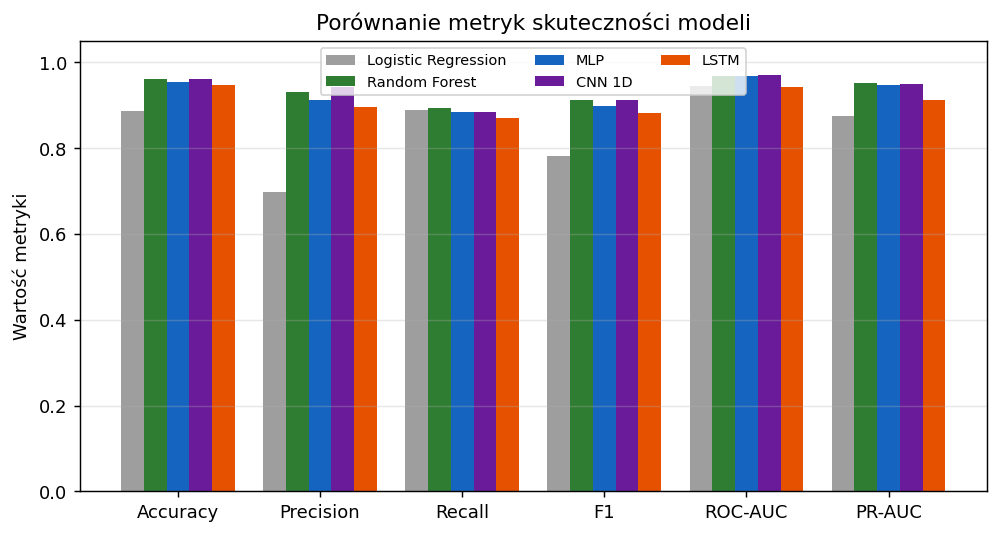
\includegraphics[width=0.82\textwidth]{metrics_comparison.png}
\caption{Porównanie metryk skuteczności modeli na zbiorze testowym.}
\label{fig:metrics}
\end{figure}

\begin{figure}[H]
\centering
\begin{minipage}{0.49\textwidth}
  \centering
  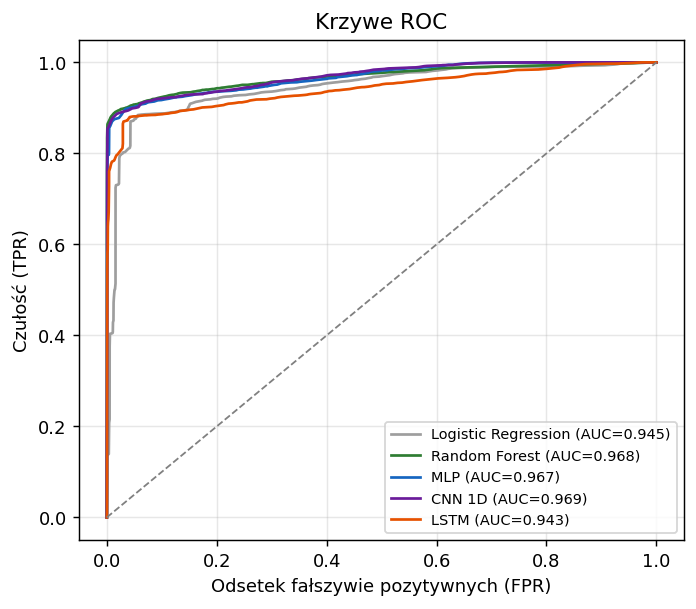
\includegraphics[width=\textwidth]{roc_curves.png}
  \caption{Krzywe ROC.}
  \label{fig:roc}
\end{minipage}\hfill
\begin{minipage}{0.49\textwidth}
  \centering
  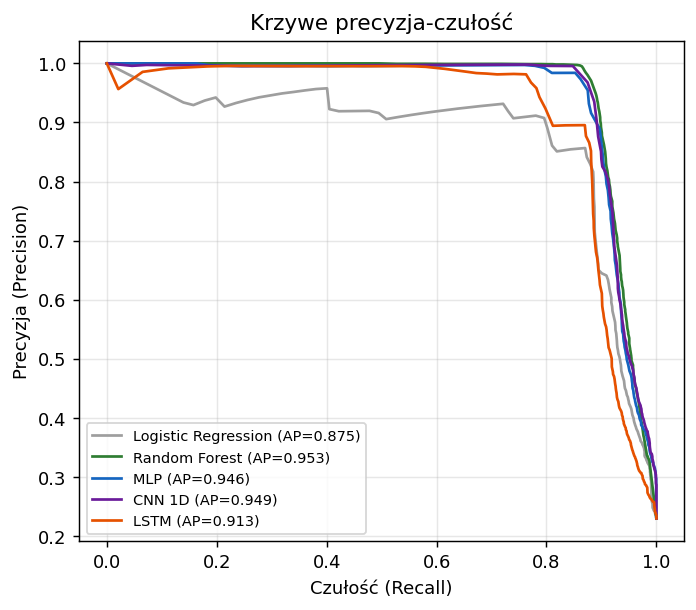
\includegraphics[width=\textwidth]{pr_curves.png}
  \caption{Krzywe precyzja--czułość.}
  \label{fig:pr}
\end{minipage}
\end{figure}

\subsection{Analiza błędów}

Macierze pomyłek (rys.~\ref{fig:cm}) pozwalają zajrzeć ,,pod maskę'' i zobaczyć,
jakie błędy popełniają modele. Las losowy wychwytuje najwięcej ataków (najwyższa
czułość), czyli rzadziej przepuszcza zagrożenie --- co w kontekście ochrony
danych jest cenne, bo przeoczone naruszenie kosztuje najwięcej. Sieć CNN z kolei
nieco rzadziej podnosi fałszywy alarm (najwyższa precyzja), czyli mniej męczy
zespół bezpieczeństwa niepotrzebnymi powiadomieniami. W praktyce ,,punkt
równowagi'' między tymi błędami można regulować progiem decyzyjnym, dopasowując
go do polityki bezpieczeństwa danej organizacji.

\begin{figure}[H]
\centering
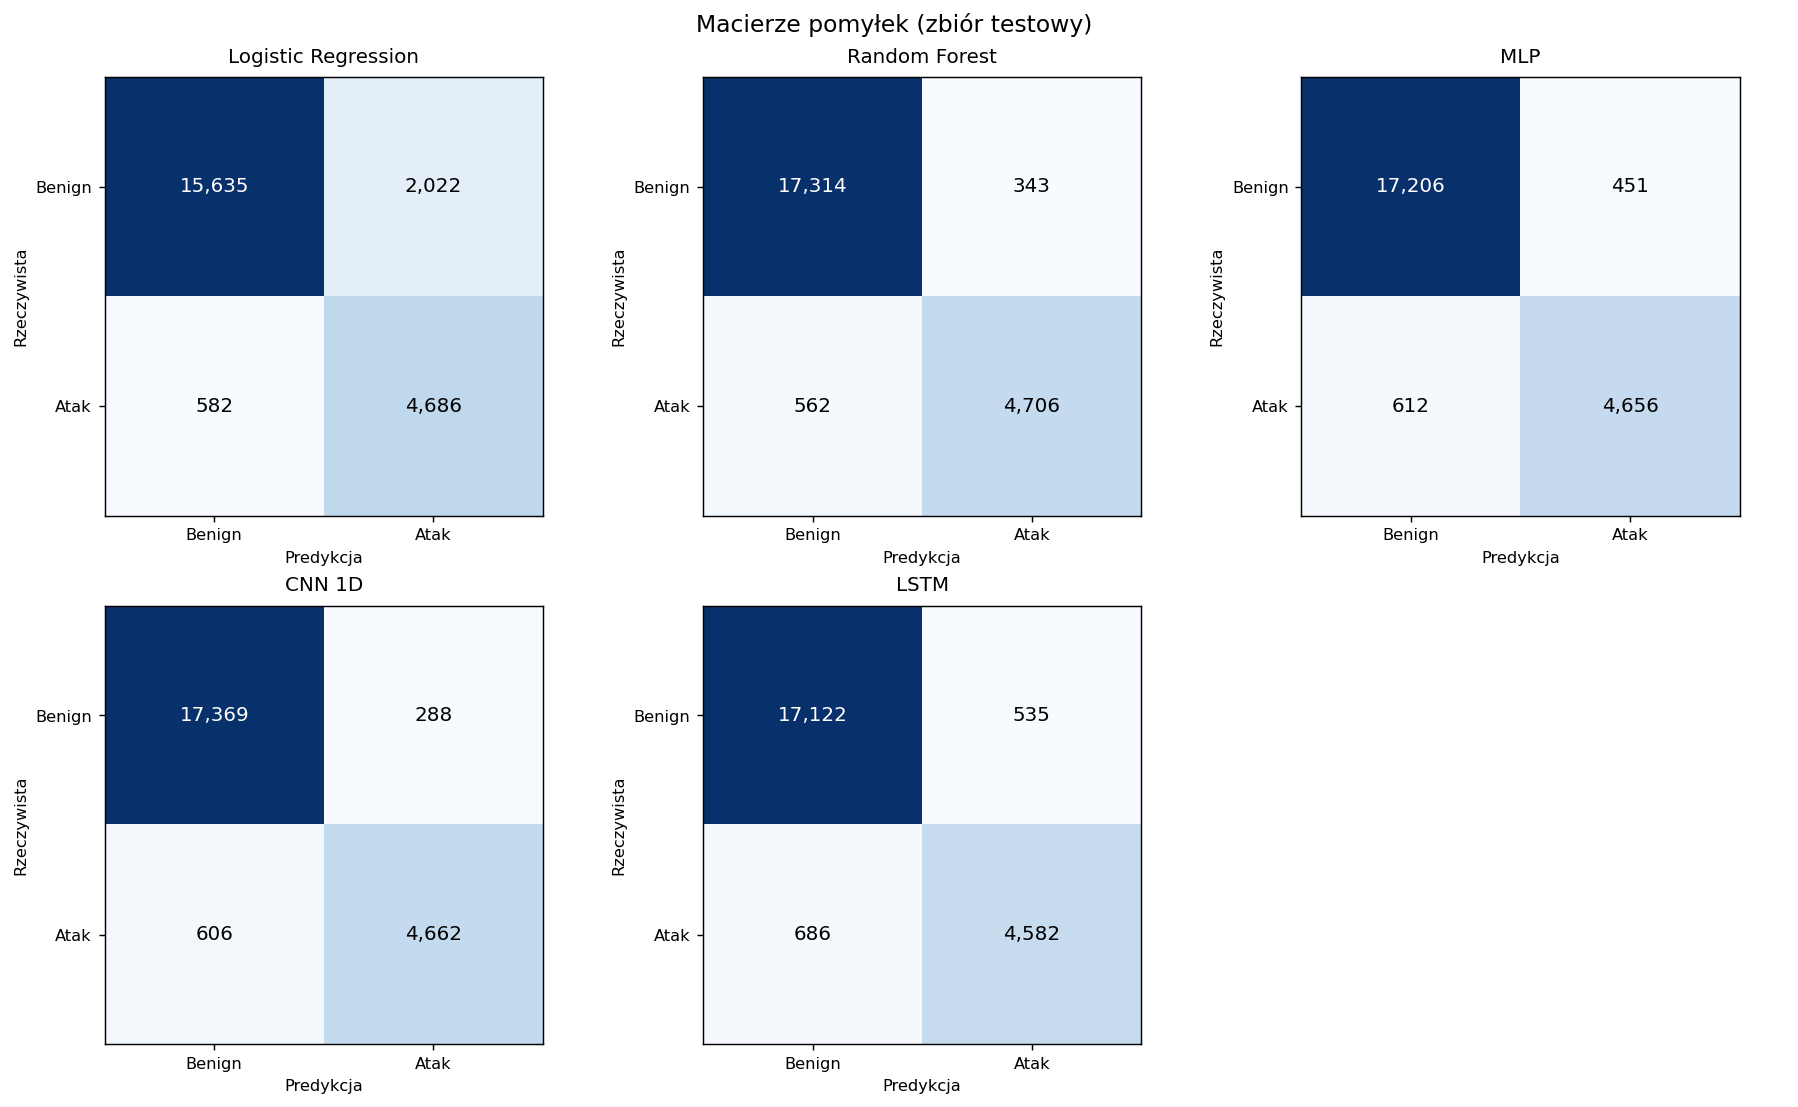
\includegraphics[width=0.82\textwidth]{confusion_matrices.png}
\caption{Macierze pomyłek na zbiorze testowym dla wszystkich modeli.}
\label{fig:cm}
\end{figure}

\subsection{Wydajność i koszt obliczeniowy}

Skuteczność to tylko jeden wymiar oceny; w środowisku chmurowym, gdzie modele
są często dotrenowywane i muszą klasyfikować ruch na bieżąco, kluczowy jest
także koszt. Tabela~\ref{tab:efficiency} zestawia czasy treningu i inferencji
oraz złożoność modeli.

\begin{table}[H]
\centering
\caption{Porównanie wydajności i złożoności modeli.}
\label{tab:efficiency}
\small
\begin{tabular}{lrrl}
\toprule
Model & Czas treningu [s] & Czas inferencji [s] & Złożoność modelu \\
\midrule
Logistic Regression & 0.78 & 0.0006 & 69 wsp. \\
Random Forest & 4.16 & 0.0801 & 300 drzew / 1\,550\,456 węzłów \\
MLP & 11.82 & 0.0281 & 17\,537 param. \\
CNN 1D & 171.74 & 0.7103 & 39\,553 param. \\
LSTM & 487.45 & 3.9718 & 134\,401 param. \\
\bottomrule
\end{tabular}
\end{table}

I tu pojawia się sedno sprawy. Las losowy uczy się w zaledwie
\resRFTrainTime~s, podczas gdy najlepszy model głęboki (\resBestDeepModel)
potrzebuje aż \resBestDeepTrainTime~s --- czyli kilkadziesiąt razy dłużej --- by
osiągnąć praktycznie ten sam wynik. Najbardziej rozbudowana sieć LSTM trenuje
się ponad osiem minut, a mimo to wypada słabiej. Również w fazie działania
(klasyfikacji nowego ruchu) las losowy i proste modele są wyraźnie szybsze od
sieci CNN i LSTM. Ten kompromis między kosztem a skutecznością dobrze obrazuje
rys.~\ref{fig:tradeoff}: najbardziej opłacalne modele leżą w lewej górnej części
wykresu --- wysoka skuteczność przy krótkim czasie uczenia.

\begin{figure}[H]
\centering
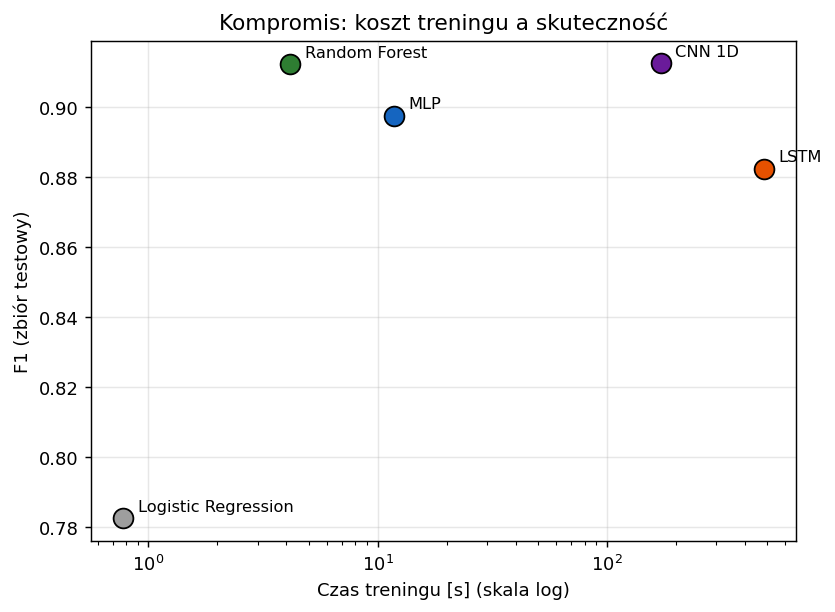
\includegraphics[width=0.8\textwidth]{time_vs_f1.png}
\caption{Kompromis między czasem treningu (skala logarytmiczna) a skutecznością
($F_1$). Modele najbardziej efektywne znajdują się w lewym górnym obszarze.}
\label{fig:tradeoff}
\end{figure}

\subsection{Przebieg uczenia modeli głębokich}

Rys.~\ref{fig:learning} przedstawia krzywe uczenia modeli głębokich: stratę
walidacyjną oraz ROC-AUC na zbiorze walidacyjnym w kolejnych epokach. Widoczna
jest stabilna zbieżność i działanie mechanizmu wczesnego zatrzymania, który
zapobiega przeuczeniu.

\begin{figure}[H]
\centering
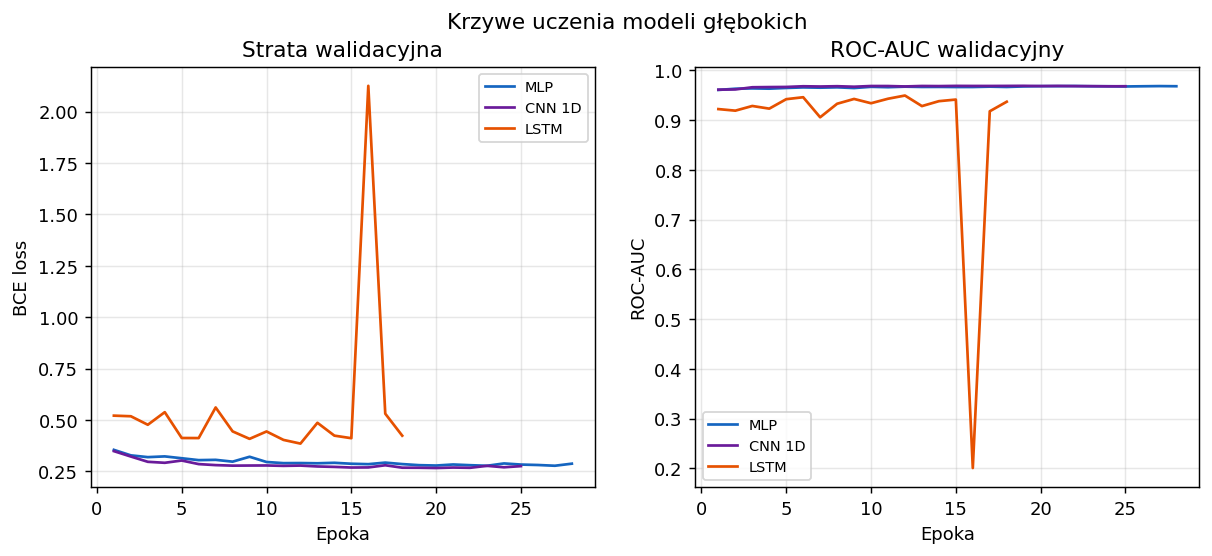
\includegraphics[width=0.88\textwidth]{learning_curves.png}
\caption{Krzywe uczenia modeli głębokich (strata i ROC-AUC walidacyjny).}
\label{fig:learning}
\end{figure}

\subsection{Interpretowalność modeli i ważność cech}

Dodatkową zaletą lasu losowego jest interpretowalność. Rys.~\ref{fig:importance}
przedstawia najważniejsze cechy według miary ważności Giniego. Pozwala to
zidentyfikować, które statystyki przepływu najsilniej różnicują ruch złośliwy i
normalny --- informacja cenna dla analityków bezpieczeństwa, a trudniej dostępna
w modelach głębokich, działających jak ,,czarna skrzynka''.

\begin{figure}[H]
\centering
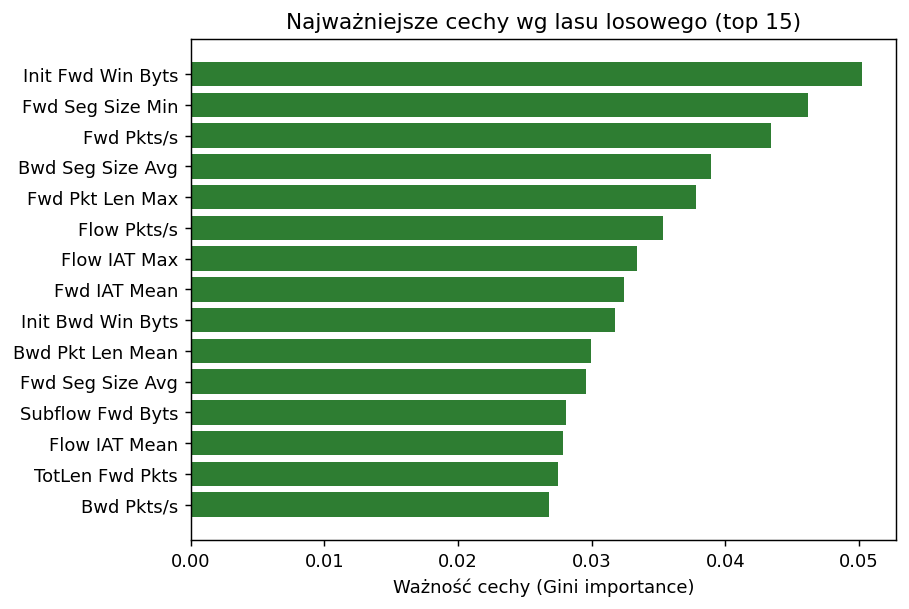
\includegraphics[width=0.8\textwidth]{feature_importance.png}
\caption{Najważniejsze cechy według lasu losowego (ważność Giniego).}
\label{fig:importance}
\end{figure}

\subsection{Podsumowanie wyników}

Zebrane wyniki pozwalają wstępnie odpowiedzieć na postawione pytania:
\begin{itemize}
  \item \textbf{Skuteczność:} las losowy i najlepszy model głęboki
        (\resBestDeepModel) są praktycznie nierozróżnialne pod względem $F_1$ i
        ROC-AUC; las losowy dodatkowo wykrywa najwięcej ataków (najwyższa
        czułość).
  \item \textbf{Koszt:} las losowy jest zdecydowanie tańszy --- uczy się
        kilkadziesiąt razy szybciej niż sieci głębokie, oferując najlepszą
        relację skuteczność--koszt.
  \item \textbf{Złożoność:} rozbudowane sieci sekwencyjne (zwłaszcza LSTM) nie
        przyniosły przewagi --- większa złożoność nie przełożyła się na lepsze
        wyniki, co potwierdza obserwacje z literatury dotyczące danych
        tabelarycznych.
\end{itemize}

\section{Wnioski końcowe}
\label{sec:wnioski}

\subsection{Podsumowanie}

W pracy zrealizowano empiryczne porównanie metod uczenia głębokiego i lasów
losowych w zadaniu prognozowania naruszeń danych w chmurze, sformułowanym jako
binarna klasyfikacja przepływów sieciowych. Zbudowano kompletny, odtwarzalny
potok obejmujący przygotowanie danych, trening pięciu modeli (regresja
logistyczna, las losowy oraz sieci MLP, CNN 1D i LSTM) oraz ich ocenę pod kątem
skuteczności i kosztu obliczeniowego.

Najważniejsze wnioski są następujące:
\begin{enumerate}
  \item \textbf{Obie rodziny metod skutecznie wykrywają naruszenia.} Zarówno las
        losowy, jak i sieci głębokie osiągają wysokie wyniki, wyraźnie
        przewyższając prosty model liniowy. To pokazuje, że złośliwa aktywność
        kryje się w złożonych zależnościach między cechami, które obie metody
        dobrze wychwytują.
  \item \textbf{Skuteczność jest niemal taka sama, ale koszt --- już nie.}
        Najlepszy model głęboki (\resBestDeepModel, $F_1 = \resBestDeepFOne$) i
        las losowy ($F_1 = \resRFFOne$) osiągają praktycznie identyczną jakość,
        przy czym las losowy dodatkowo wykrywa najwięcej ataków (najwyższa
        czułość), uczy się kilkadziesiąt razy szybciej i potrafi wskazać, które
        cechy zaważyły na decyzji. To czyni go wyjątkowo atrakcyjnym wyborem.
  \item \textbf{Bardziej skomplikowane nie znaczy lepsze.} Rozbudowane sieci
        sekwencyjne (zwłaszcza LSTM) nie przewyższyły ani lasu losowego, ani
        prostszej sieci, generując jedynie wyższy koszt. Potwierdza to znaną z
        literatury obserwację, że dla danych w postaci tabeli metody oparte na
        drzewach pozostają bardzo trudne do pobicia.
  \item \textbf{Wybór metody zależy od kontekstu.} Jeśli liczą się szybkie
        dotrenowywanie, niski koszt, dobra wykrywalność i zrozumiałość decyzji
        --- las losowy jest naturalnym wyborem. Sieci głębokie warto rozważyć
        tam, gdzie zależy nam na maksymalnym ograniczeniu fałszywych alarmów
        (wysoka precyzja CNN) i dysponujemy większymi zasobami obliczeniowymi.
\end{enumerate}

\subsection{Ograniczenia}

Wyniki należy interpretować w świetle ograniczeń pracy:
\begin{itemize}
  \item Eksperyment przeprowadzono na losowym podzbiorze danych
        \texttt{\resDataSource} (ze względu na rozmiar pełnego zbioru liczącego
        kilka gigabajtów). Większa próbka mogłaby nieco zmienić konkretne
        liczby, choć raczej nie ogólne wnioski; program jest gotowy do
        uruchomienia na pełnym zbiorze bez zmian w kodzie.
  \item Nie przeprowadzono wyczerpującego strojenia hiperparametrów --- użyto
        rozsądnych wartości domyślnych, jednakowych dla wszystkich modeli.
  \item Obliczenia prowadzono na CPU; na akceleratorach GPU względne czasy
        treningu modeli głębokich uległyby skróceniu, choć relacja kosztów
        pozostałaby jakościowo podobna.
  \item Zadanie ograniczono do klasyfikacji binarnej; analiza wieloklasowa
        (rozróżnianie typów ataków) stanowi naturalne rozszerzenie.
\end{itemize}

\subsection{Kierunki dalszych prac}

Możliwe rozszerzenia obejmują: (1) walidację na pełnym zbiorze CSE-CIC-IDS2018 i
innych zbiorach (UNSW-NB15, NSL-KDD); (2) systematyczne strojenie
hiperparametrów oraz włączenie metod gradient boosting (XGBoost, LightGBM);
(3) klasyfikację wieloklasową i wykrywanie nieznanych ataków metodami
półnadzorowanymi; (4) analizę odporności modeli na ataki adwersarialne oraz
dryf danych; (5) integrację najlepszego modelu w architekturze strumieniowej
(np.\ przetwarzanie przepływów w czasie rzeczywistym) wraz z mechanizmami
wyjaśnialności (SHAP) dla wsparcia analityków SOC.

\subsection{Podsumowanie końcowe}

Przeprowadzone badanie pokazuje, że w prognozowaniu naruszeń danych w chmurze
nie ma jednej, bezdyskusyjnie najlepszej metody --- wybór jest kompromisem
między skutecznością a kosztem, szybkością i zrozumiałością decyzji. Dla danych
opisujących ruch sieciowy las losowy okazuje się wyjątkowo silnym i tanim
rozwiązaniem, któremu sieci głębokie co najwyżej dorównują, lecz go nie
prześcigają --- i to dopiero za cenę znacznie większego nakładu obliczeniowego.
Dla studenta czy inżyniera bezpieczeństwa płynie z tego praktyczny wniosek:
zanim sięgnie się po skomplikowane sieci neuronowe, warto najpierw wypróbować
dobrze dobraną metodę klasyczną.


\newpage
\bibliographystyle{plain}
\bibliography{bibliografia}

\end{document}
